\documentclass{article}
\usepackage[margin=1.5cm,bottom=2cm]{geometry}
\usepackage{fancyhdr}
\usepackage{graphicx}
\pagestyle{fancy}
\usepackage{amsmath}

\begin{document}
%\fancyhead[L]{ 
\includegraphics[width=2cm]{/Users/tjwilli/google_drive/course_materials/global/au_logo.png} }
\fancyhead[R]{PHYS 2250: General Physics II}
\fancyfoot[C]{\thepage}
\vspace*{0cm}
\begin{center}
	{\LARGE \textbf{Quiz 6}}\\
	\vspace{0.25cm}
	%{\Large Vector Review (Ungraded)}\\
	\vspace{0.25cm}
%	{\Large Friday, September 17}
\end{center}
%The following information may or may not be of use:\\
%\hrulefill\\
\begin{align*}
	\text{Magnitude of electron charge:}\ e&=1.6\times10^{-19}\ \mathrm{C}\\
	\text{Electron current:}\ i&=nA\overline{v}\\
	\text{Electron drift velocity:}\ \overline{v}=uE\\
%	\text{Conventional current:}\ I&=\left|q\right|i\\
%	\text{Bio-Savart:}\ 
%	\Delta \vec{B}&=\frac{\mu_0}{4\pi}\frac{I\Delta\vec{l}\times \hat{r}}{r^2}\\
%	\text{Straight Wire:}\ \left|\vec{B}\right|&=\frac{\mu_0}{4\pi}\frac{LI}{r\sqrt{r^2+\left(L/2\right)^2}}\\
%	\text{Very long straight wire:}\ \left|\vec{B}\right|&\approx \frac{\mu_0}{4\pi}\frac{2I}{r}\\
%	\text{Center of loop of current: }\ \left|\vec{B}\right|&=\frac{\mu_0}{4\pi}\frac{2\pi R^2I}{\left(z^2+R^2\right)^{3/2}}
\end{align*}

%\hrulefill \\
%\\
In the figure below, the thin resistor is made out of the same material as the connecting wires (Nichrome). You know the following information:
\begin{itemize}
	\item The emf $\varepsilon$ of the battery is 1.5 V
	\item The length $L$ of each conducting wire is 0.5 cm
	\item The length $L_R$ of the resistor is 0.1 cm
	\item The cross-sectional area of each conducting wire is 0.3 mm$^2=3\times10^{-7}\ \mathrm{m}^2$
	\item The cross-sectional area of the resistor is 0.005 mm$^2=5\times10^{-9}\ \mathrm{m}^2$
\end{itemize}
You also know the conductive properties of Nichrome:
	\begin{table}[ht]
	\centering
	\begin{tabular}{|c|c|}
		\hline
		\textbf{Property} & \textbf{Value} \\
		\hline
		Electron density ($n$) & $9\times10^{28}\ \mathrm{m}^{-3}$\\
		\hline 
		Electron mobility ($u$) & $7\times10^{-5}\ \frac{\mathrm{m}/\mathrm{s}}{\mathrm{N}/\mathrm{C}}$\\
		\hline 
		Charge carrier & electron \\
		\hline
	\end{tabular}
	\caption{}
	\label{tab1}
\end{table}
\begin{center}
	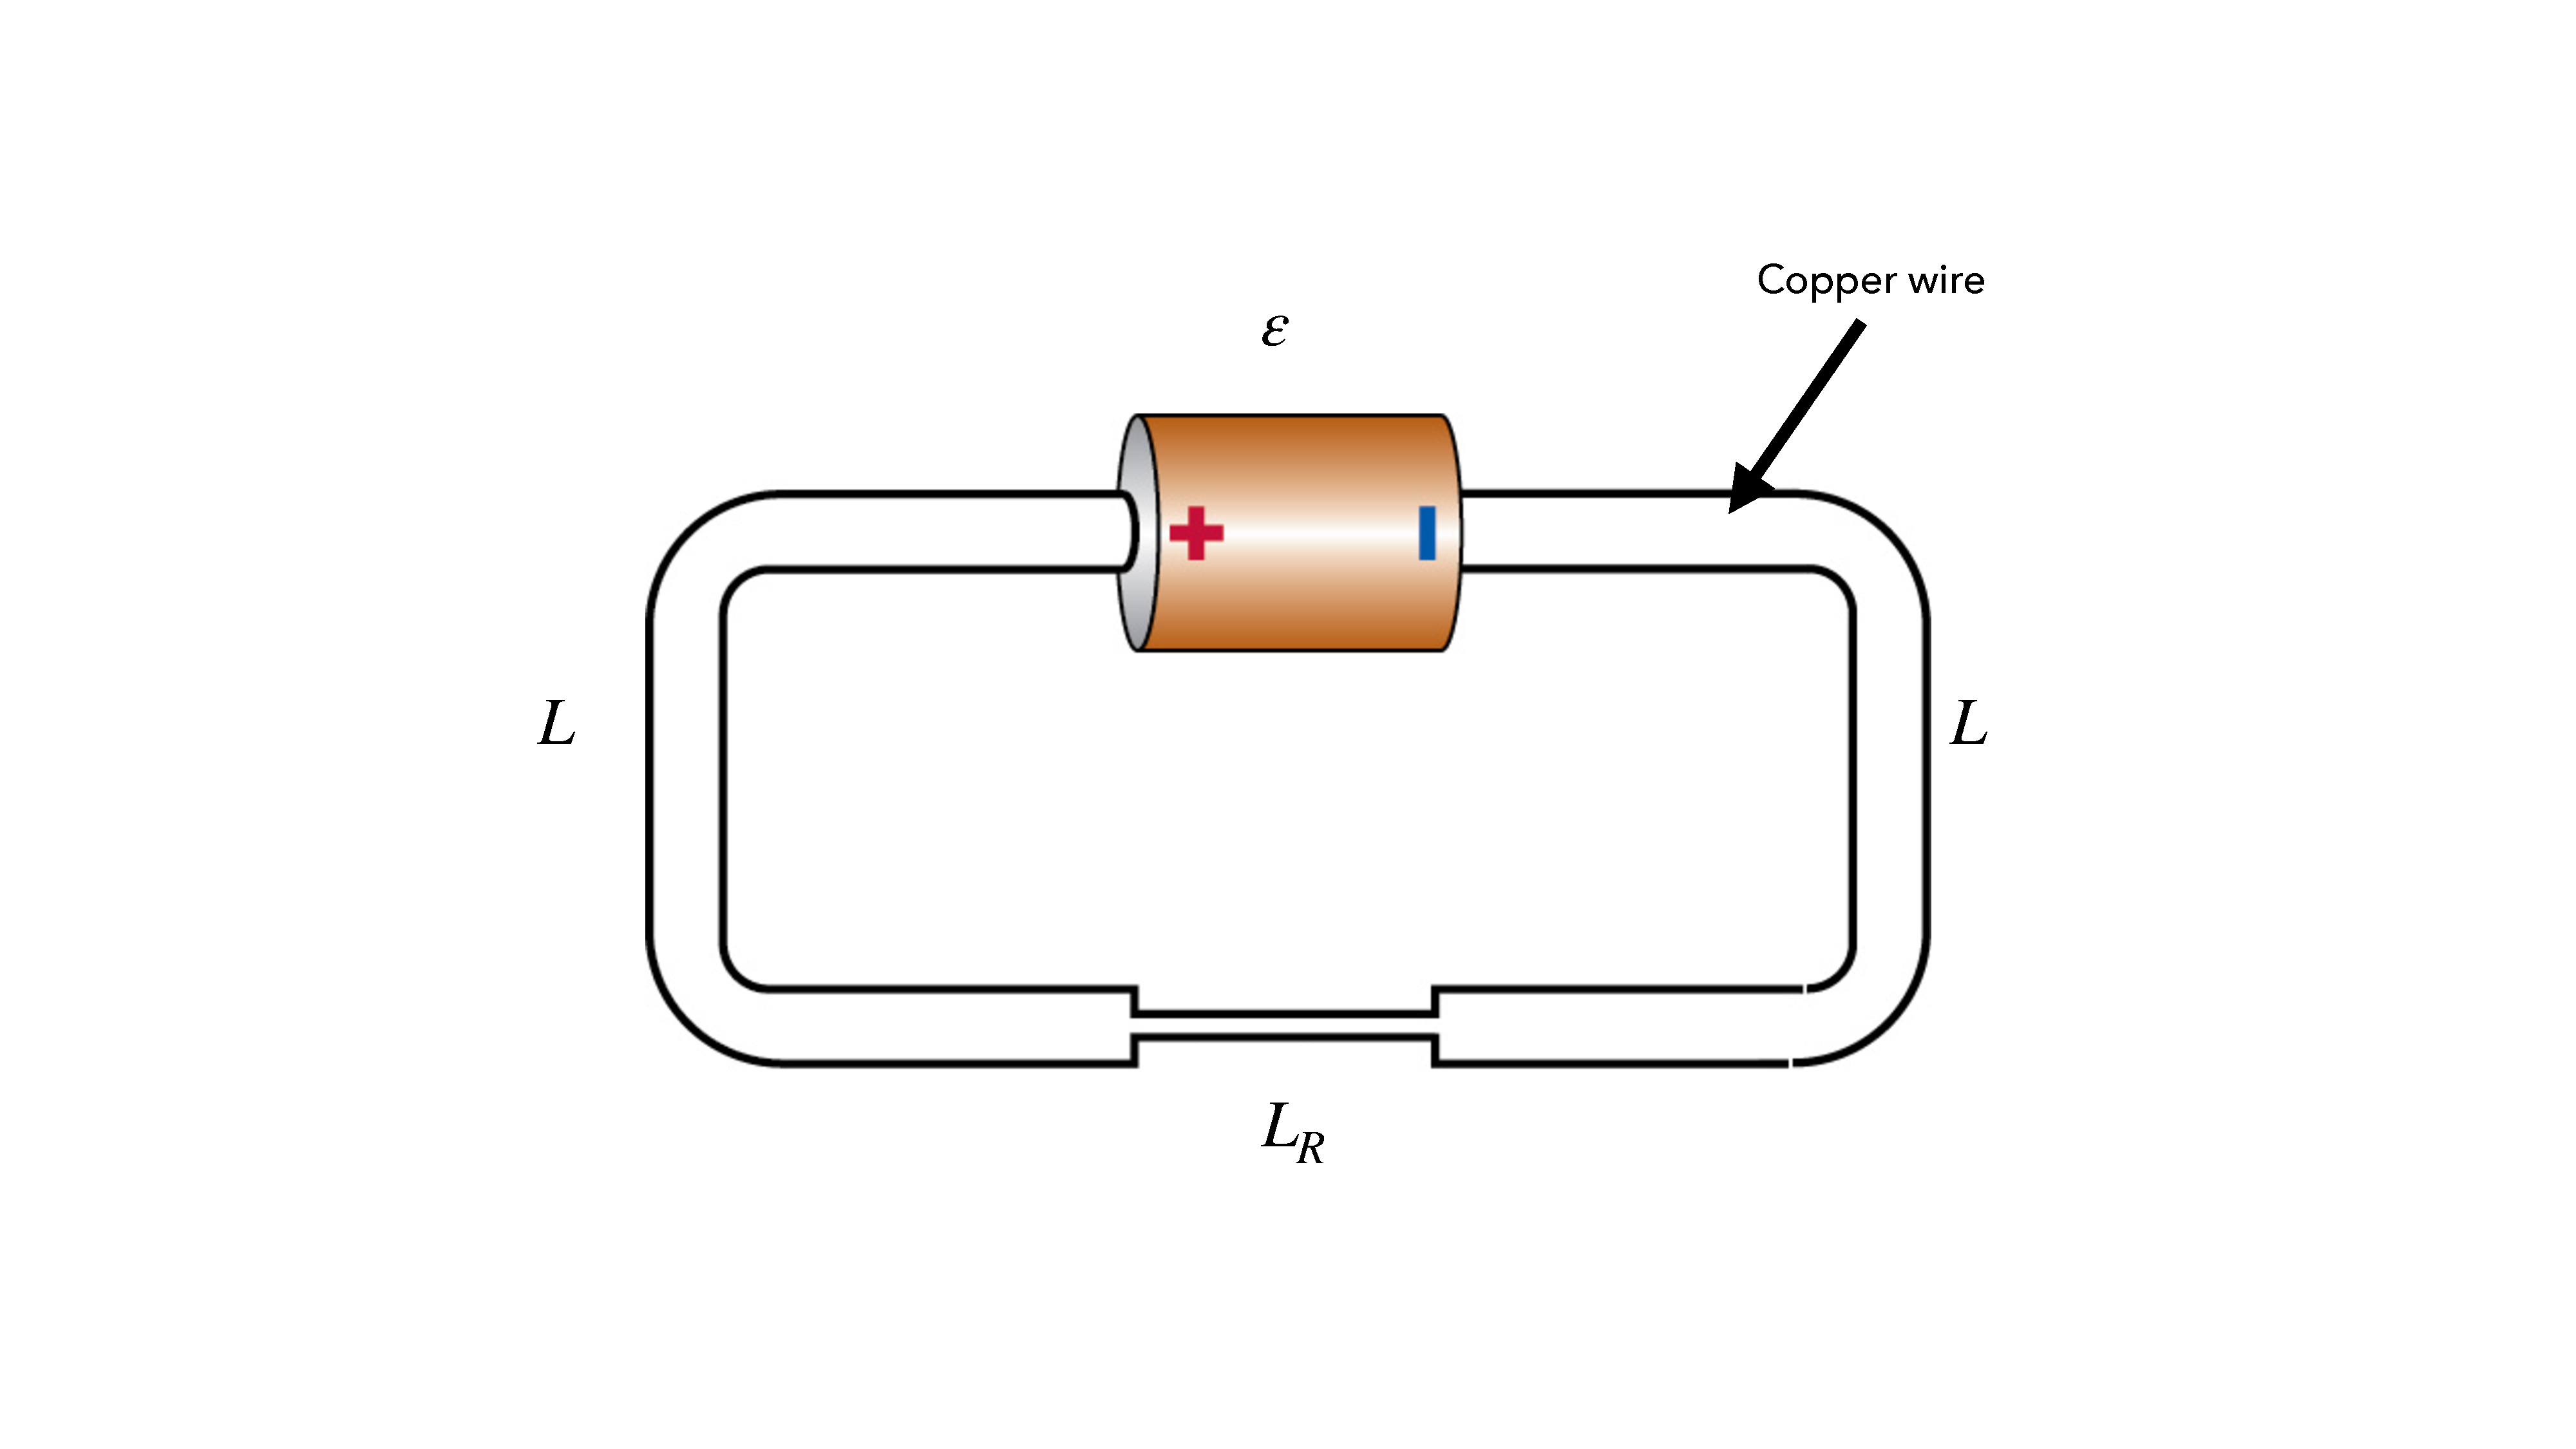
\includegraphics[width=.5\textwidth]{thin_resistor_quiz}
\end{center}

What is the (a) Electric field and (b) electron drift velocity inside of the thin resistor?
\end{document}